%%%%%%%%%%%%%%%%%%%%%%%%%%%%%%%%%%%%%%%%%
% Proceedings of the National Academy of Sciences (PNAS)
% LaTeX Template
% Version 1.0 (19/5/13)
%
% This template has been downloaded from:
% http://www.LaTeXTemplates.com
%
% Original author:
% The PNAStwo class was created and is owned by PNAS:
% http://www.pnas.org/site/authors/LaTex.xhtml
% This template has been modified from the blank PNAS template to include
% examples of how to insert content and drastically change commenting. The
% structural integrity is maintained as in the original blank template.
%
% Original header:
%% PNAStmpl.tex
%% Template file to use for PNAS articles prepared in LaTeX
%% Version: Apr 14, 2008
%
%%%%%%%%%%%%%%%%%%%%%%%%%%%%%%%%%%%%%%%%%

%----------------------------------------------------------------------------------------
%	PACKAGES AND OTHER DOCUMENT CONFIGURATIONS
%----------------------------------------------------------------------------------------

%------------------------------------------------
% BASIC CLASS FILE
%------------------------------------------------

%% PNAStwo for two column articles is called by default.
%% Uncomment PNASone for single column articles. One column class
%% and style files are available upon request from pnas@nas.edu.

%\documentclass{pnasone}
\documentclass{pnastwo}

%------------------------------------------------
% POSITION OF TEXT
%------------------------------------------------

%% Changing position of text on physical page:
%% Since not all printers position
%% the printed page in the same place on the physical page,
%% you can change the position yourself here, if you need to:

% \advance\voffset -.5in % Minus dimension will raise the printed page on the 
                         %  physical page; positive dimension will lower it.

%% You may set the dimension to the size that you need.

%------------------------------------------------
% GRAPHICS STYLE FILE
%------------------------------------------------

%% Requires graphics style file (graphicx.sty), used for inserting
%% .eps/image files into LaTeX articles.
%% Note that inclusion of .eps files is for your reference only;
%% when submitting to PNAS please submit figures separately.

%% Type into the square brackets the name of the driver program 
%% that you are using. If you don't know, try dvips, which is the
%% most common PC driver, or textures for the Mac. These are the options:

% [dvips], [xdvi], [dvipdf], [dvipdfm], [dvipdfmx], [pdftex], [dvipsone],
% [dviwindo], [emtex], [dviwin], [pctexps], [pctexwin], [pctexhp], [pctex32],
% [truetex], [tcidvi], [vtex], [oztex], [textures], [xetex]

\usepackage{graphicx}
\usepackage{amsmath}
\usepackage{float}

%------------------------------------------------
% OPTIONAL POSTSCRIPT FONT FILES
%------------------------------------------------

%% PostScript font files: You may need to edit the PNASoneF.sty
%% or PNAStwoF.sty file to make the font names match those on your system. 
%% Alternatively, you can leave the font style file commands commented out
%% and typeset your article using the default Computer Modern 
%% fonts (recommended). If accepted, your article will be typeset
%% at PNAS using PostScript fonts.

% Choose PNASoneF for one column; PNAStwoF for two column:
%\usepackage{PNASoneF}
%\usepackage{PNAStwoF}

%------------------------------------------------
% ADDITIONAL OPTIONAL STYLE FILES
%------------------------------------------------

%% The AMS math files are commonly used to gain access to useful features
%% like extended math fonts and math commands.

\usepackage{amssymb,amsfonts,amsmath}

%------------------------------------------------
% OPTIONAL MACRO FILES
%------------------------------------------------

%% Insert self-defined macros here.
%% \newcommand definitions are recommended; \def definitions are supported

%\newcommand{\mfrac}[2]{\frac{\displaystyle #1}{\displaystyle #2}}
%\def\s{\sigma}

%------------------------------------------------
% DO NOT EDIT THIS SECTION
%------------------------------------------------

%% For PNAS Only:
\contributor{Submitted to Proceedings of the National Academy of Sciences of the United States of America}
%\url{www.pnas.org/cgi/doi/10.1073/pnas.0709640104}
\copyrightyear{2015}
\issuedate{03-16-2015}
\volume{1}
\issuenumber{1}

%----------------------------------------------------------------------------------------

\begin{document}

%----------------------------------------------------------------------------------------
%	TITLE AND AUTHORS
%----------------------------------------------------------------------------------------

\title{Multifactor, multiple people. Authentication approach for unlocking encrypted files.} % For titles, only capitalize the first letter

%------------------------------------------------

\author{Yuri Gorokhov\affil{1}{University of California, San Diego},
Lars Noergaard Nielsen\affil{1}{University of California, San Diego}}

\contributor{Submitted as part of graduate security course CSE227.}

%----------------------------------------------------------------------------------------

\maketitle % The \maketitle command is necessary to build the title page

\begin{article}

%----------------------------------------------------------------------------------------
%	ABSTRACT, KEYWORDS AND ABBREVIATIONS
%----------------------------------------------------------------------------------------

\begin{abstract}
Proposal of a system to authenticate access to encrypted files using both Multifactor and multiple people, across different locations. Making sure that files are only accessible with the consent of all involved participants.
\end{abstract}

%------------------------------------------------

\keywords{Multifactor | Encryption} % When adding keywords, separate each term with a straight line: |

%------------------------------------------------

%----------------------------------------------------------------------------------------
%	PUBLICATION CONTENT
%----------------------------------------------------------------------------------------

%% The first letter of the article should be drop cap: \dropcap{} e.g.,
%\dropcap{I}n this article we study the evolution of ''almost-sharp'' fronts

\section{Introduction}

\dropcap{Q}uorum \( \rightarrow \) the minimum number of members of an assembly or society that must be present at any of its meetings to make the proceedings of that meeting valid.

Controlling who has access to files is often a requirement in industry and various other contexts. Systems for dealing with information that only is accessible with multiple people's consent is therefore interesting to investigate. Software for file access control purposes include Dell Identity Manager\cite{CLAcha1}, User Lock Access Manager \cite{UserLock} and native OS support such as an Access Control List. These systems is not addressing security as such, as not providing encryption capabilities. Common for these solutions is that file access is administered centrally by an administrator. We propose an approach were users actively set file permissions by agreeing to encrypt files by their common consent, only allowing access to these files when all parties have responded to the access request. The latter step is additionally secured by MultiFactor Authentication.

\section{Multifactor authorization: Yubikey}

Yubikey is a marketed USB dongle used for various Multifactor authentication purposes. It can be set up in different modes, for One Time Password (OTP) based on a series of variables, including sequence numbers. In this work we used the Challenge-Response mode, where the Yubikey is configured with a shared Secret Key among the server and the key itself. The Secret Key is SHA-1 cryptographic hash function. 

Yubikey furthermore provides a simple procedure for the user: only a physical touch on the device is necessary to allow the device to respond to the presented challenge.


\section{System Description}

The proposed system is composed of a user client, hard drive client and a verification server. The user clients forms a quorum that can respond to request from harddrive clients to unlock files. The basic idea is for server and userclients be initiated with a shared secret \ref{basicSystemFigure}.

A benefit from this central point of control is that the server can deny access to a file, even though participants grant access, which might be useful in some access schemes.

Donec nec egestas ipsum. Nullam vel felis quis libero ullamcorper sagittis bibendum nec est. Ut eu interdum urna. Ut aliquam orci non massa rutrum aliquam. Suspendisse rhoncus, ex at tincidunt varius, risus nisl iaculis erat, et tempus felis eros non purus. Quisque varius, velit molestie fermentum tincidunt, purus dolor lobortis erat, in consectetur dui libero et tortor. Etiam a quam dui. Mauris pulvinar, sem vitae ullamcorper porta, est augue luctus sapien, at ultricies purus neque sed massa. Integer aliquam placerat dignissim. Curabitur imperdiet nisl ac ullamcorper porttitor. Sed pharetra libero et magna consequat placerat sit amet sed purus. Vivamus et maximus libero. Morbi auctor in sapien placerat molestie. Maecenas maximus tempus sapien nec scelerisque. Nam id commodo dolor.

\begin{figure}[H]
\centerline{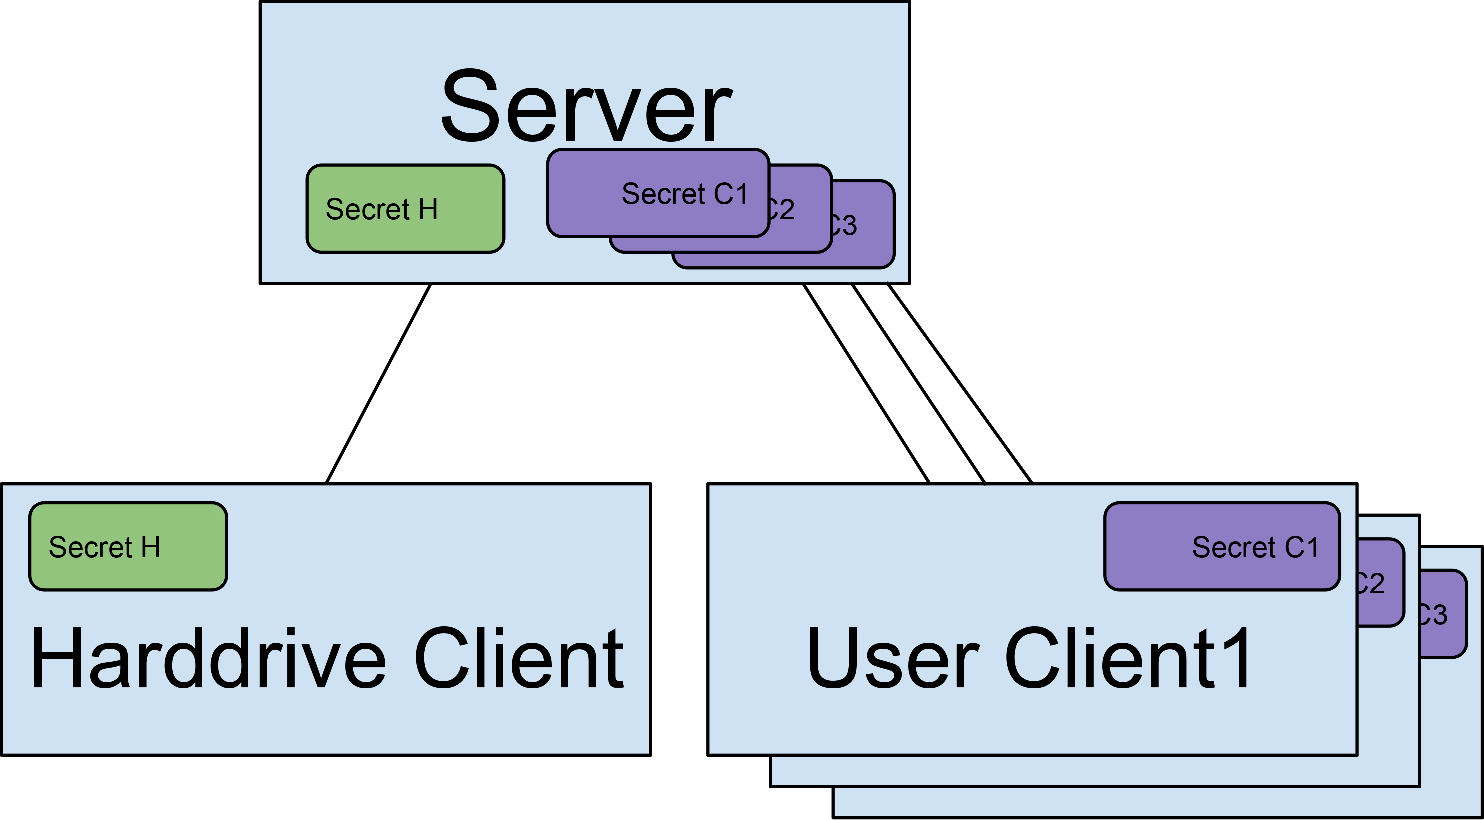
\includegraphics[width=1\linewidth]{images/BasicSystem.pdf}}
\caption{System components and interaction. 4 major steps to grant access.}\label{basicSystemFigure}
\end{figure}

\begin{figure}[H]
\centerline{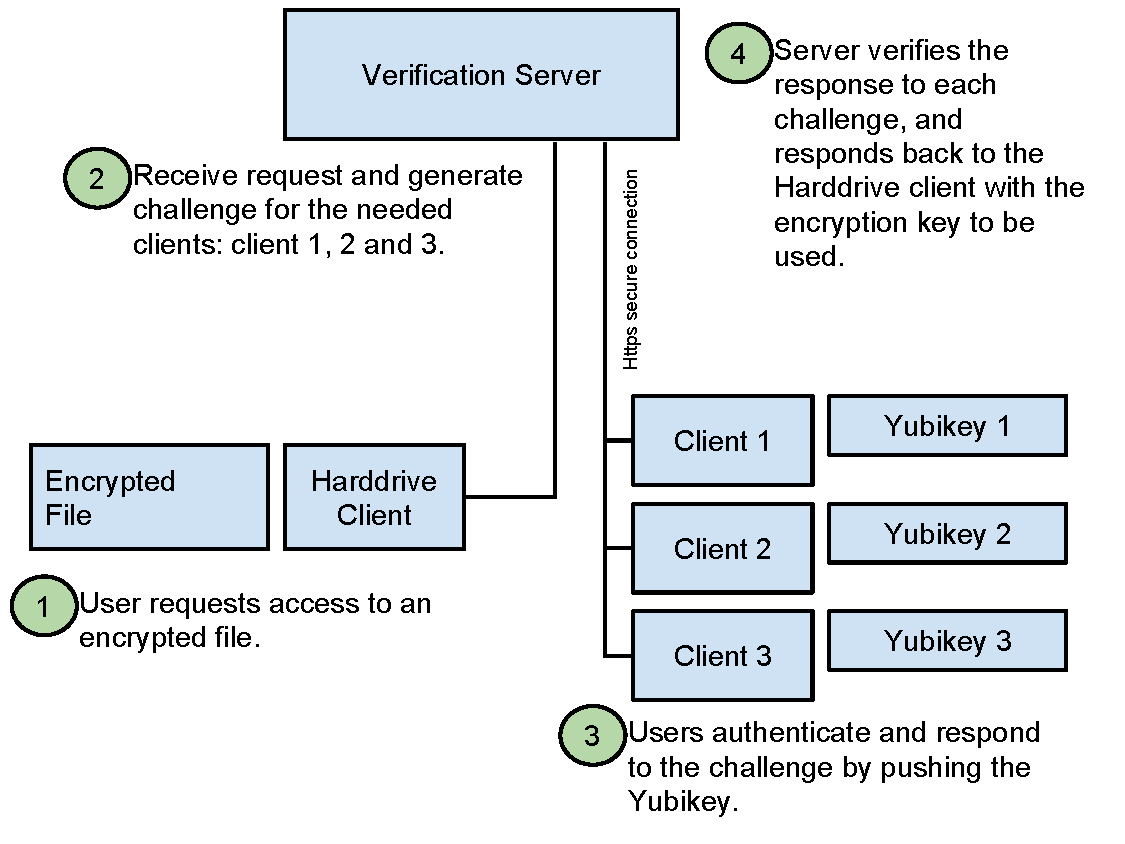
\includegraphics[width=1\linewidth]{SystemFigure.pdf}}
\caption{System components and interaction. 4 major steps to grant access.}\label{systemfigure}
\end{figure}

\section{Previous work}
We based our model on a proposed hard drive encryption mechanism published on the Yubikey website\cite{YubikeyEncryption}. In their proposed configuration the Yubikey is programmed with a secret key after which it is able to perform HMAC-SHA1 encryption. The device is said to be operating in Challenge-Response mode since you can send it a challenge and it will respond with the HMAC-SHA1 encryption of the challenge with the secret key. This is depicted in figure 1.


\begin{figure}[H]
\centerline{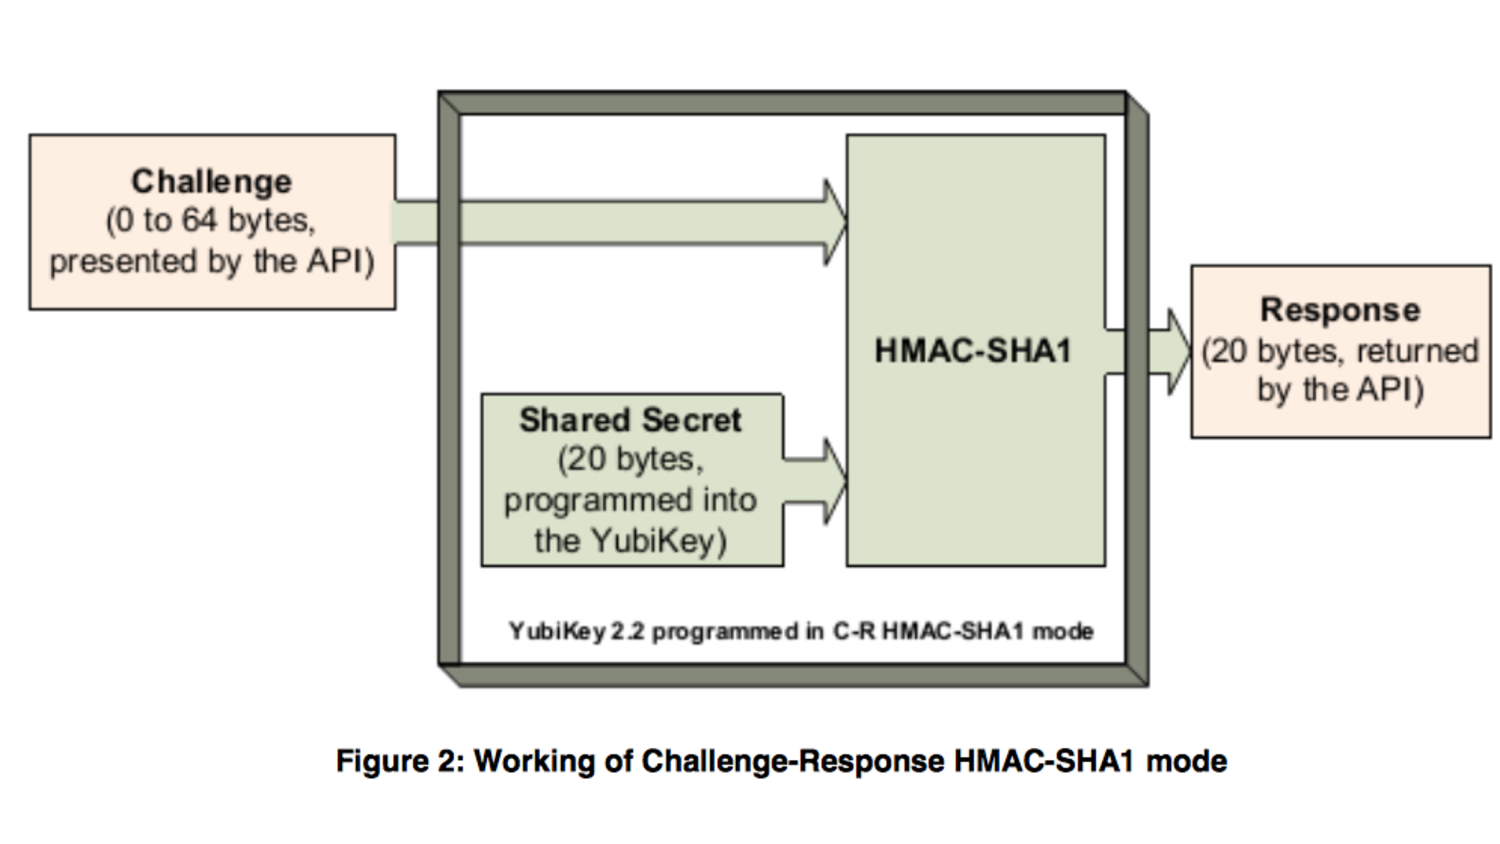
\includegraphics[width=0.7\linewidth]{ChallengeResponseFigure.pdf}}
\caption{Challenge-Response mode of Yubikey.}\label{systemfigure}
\end{figure}

Figure 2 shows how this mode is used for encrypting a local hard drive. The hard drive is encrypted with a Drive Encryption Key (DEK) which is stored in a table along with the secret. Both are encrypted using AES. The key used for the encryption is shown in Figure 2. Once the user enters his password a challenge is generated. The challenge consists of the password itself and a sequence number (Seq) that is also stored in the table. This challenge is sent to the Yubikey, whose response allows us to decrypt the DEK and the secret. The hard drive can now be decrypted. After decryption the DEK is re-encrypted with a new sequence number and the secret.

\begin{figure}[H]
\centerline{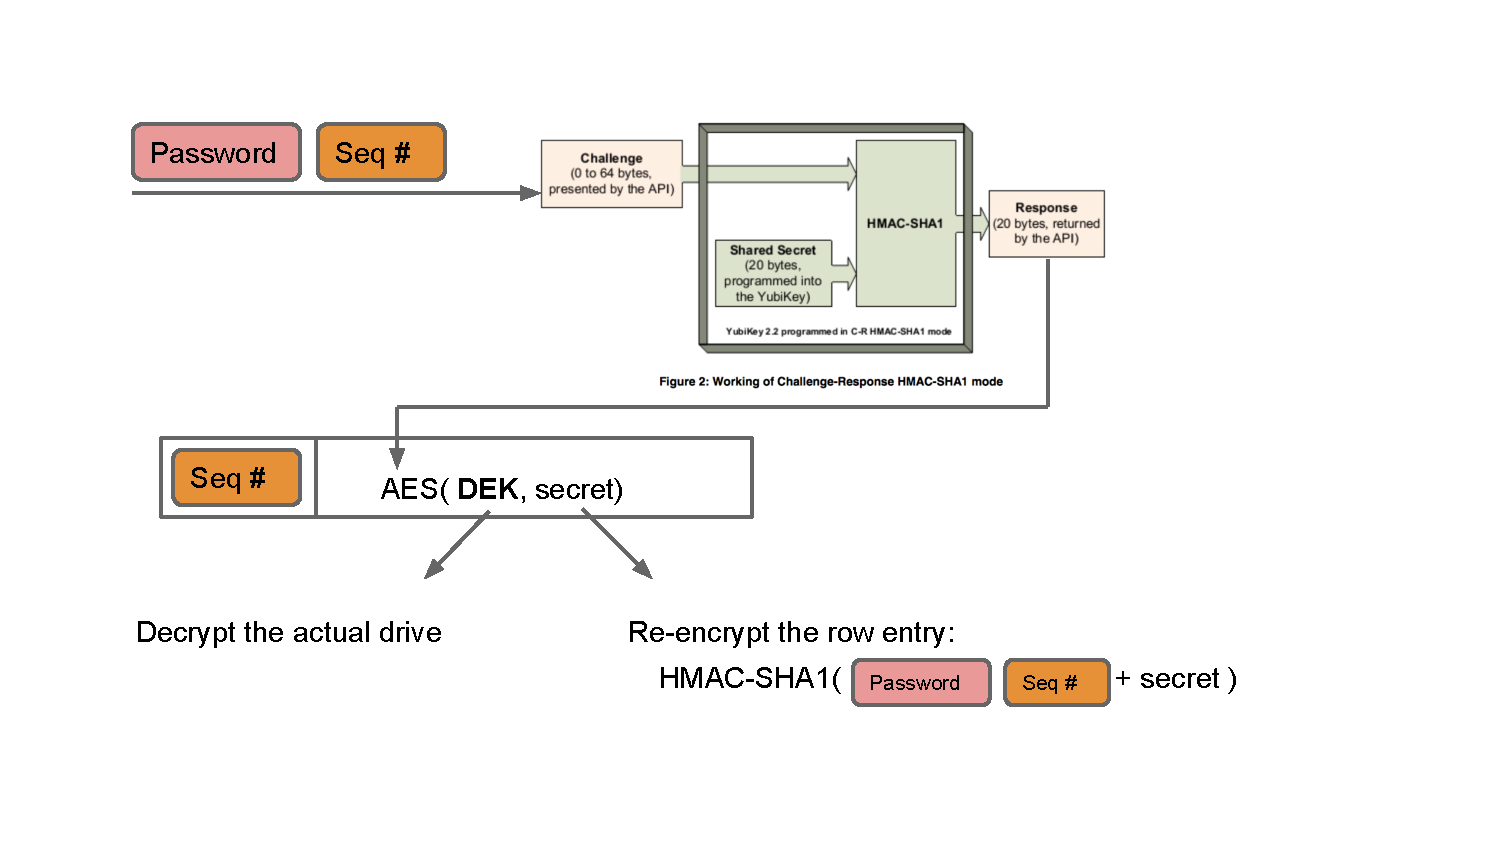
\includegraphics[width=1\linewidth]{HardDriveEncryptionFigure.pdf}}
\caption{Local hard drive encryption configuration.}\label{systemfigure}
\end{figure}

%------------------------------------------------




\section{Encryption scheme}

This sections presents the encryption scheme used, to ensure that decryption of the file is only possible when responses from all participants and their Yubikey challenges are retrieved. 

\subsection{Setup Of Quorum}

When a user is added to the server, he is given a secret key by the server that is written into the Yubikey. 

The hard drive host (the client program that is in charge of decrypting the drive) generates a Drive Encryption Key (DEK) to encrypt the hard drive with. Once encrypted, it sends a request to the server to set up a quorum of users with which it wants to share the encryption with. The server responds with an encryptionId and a secret cryptographic hash \( SHA(\sum key) \). This hash, along with the DEK are AES-encrypted and stored on the hard drive host. The key used for the encryption is calculated as follows:
\begin{equation}
	key = HMACSHA1( challenge, SHA(\sum key))
\end{equation}
\begin{equation}
	challenge = SHA(encryptionId + seq + password)
\end{equation}
The seq is a sequence number that is used to provide entropy to the challenge, it is also stored on the host. The password is necessary to generate the challenge in the future, and is global to this hard drive, not specific to any particular user in the quorum. After this encryption the hard drive host no longer has access to the DEK or the \( SHA(\sum key) \).

During the setup phase the server generates a key for each user in the quorum that is unique for the user-encryptionId pair. These keys comprise the \( SHA(\sum key) \) cryptographic hash used above. Each of these keys is stored on the server 

\section{Security Evaluation}
We evaluate the security of the proposed system by considering various attack vectors. We leave the evaluation of specific encryption and hashing mechanisms to other work, and assume them to be computationally unreasonably hard to break. We also do not evaluate the security implications of specifically using the Yubikey product, Yubico provides a detailed evaluation on their website \cite{YubikeySecurity}. 

\subsection{Server Attacks}
In designing the server side component we took deliberate care not to expose enough information to compromise the security of the hard drive at any point in the future. The database on the server stores the following items:
\begin{itemize}
	\item Yubikey secret of each user (AES encrypted)
	\item Key that corresponds to the user's share of an encrypted hard drive (AES encrypted)
	\item Mapping of hard drive to users who belong to the encryption
	\item Sequence number used for obfuscation
\end{itemize}
In order to decrypt the secret or the key, the attacker would need to gain access to the user's secret in order to be able to generate the decryption key via a HMAC-SHA1 algorithm. While the server does not provide any additional protection if the user secret has been compromised, it does not make matters any worse. Furthermore all users of a particular hard drive would need to be compromised in this way for a successful decryption. This is analogous to finding out everyone's password, which is stored on their YubiKey device.

\subsection{Network Attacks}
All communications are assumed to be SSL encrypted in a production environment to provide the first layer of security. With that in mind, let us consider what data is sent over the network during the decryption process.

\subsubsection{Between Client and Server}
When the client initiates a decryption, it sends over an \textbf{encryptionId} and a challenge. The encryptionId which is used to identify the hard drive and associated users. The challenge is a SHA hash of the encryptionId, a sequence number (seq) and an optional password. Finally the server will answer with a response.
\begin{itemize}
	\item encryptionId
	\item challenge \( \Rightarrow  SHA(encryptionId, seq, password) \)
	\item response \( \Rightarrow HMACSHA1(challenge, SHA( \sum Keys)) \)
\end{itemize}
The challenge and the response leak no data, nor are they useful in a future decryption attempt since the sequence number will have changed. The encryptionId is in itself not of much use, however if somebody had also access to the server database, they would be able to find out which users are participating in a decryption. Even then, they would still need to attain the secret's of all the users to be able to decrypt their keys.

\subsubsection{Between Server and Users}
Between the server and users, only challenge and response are exchanged over the wire. These change every request due to per-user sequence numbers thus intercepting these would not lead to future vulnerabilities.

\subsection{Hard Drive host attacks}
\subsection{Client User Attacks}

%------------------------------------------------

\section{Discussion}

Discussion on strengths and weaknesses of the solution

%----------------------------------------------------------------------------------------
%	ACKNOWLEDGEMENTS
%----------------------------------------------------------------------------------------

\pagebreak

\begin{acknowledgments}
This work was supported by..
\end{acknowledgments}

%----------------------------------------------------------------------------------------
%	BIBLIOGRAPHY
%----------------------------------------------------------------------------------------

\begin{thebibliography}{10}


\bibitem{UserLock}
http://www.isdecisions.com/lp/userlock/userlock-windows-network-security.htm?gclid=CMfPl-rqisQCFciBfgodhxwAmQ

\bibitem{CLAcha1}
http://software.dell.com/products/identity-manager-data-governance/

\bibitem{YubikeyEncryption}
https://www.yubico.com/applications/disk-encryption/full-disk-encryption/

\bibitem{YubikeySecurity}
https://www.yubico.com/wp-content/uploads/2012/10/Security-Evaluation-v2.0.1.pdf

\end{thebibliography}

%----------------------------------------------------------------------------------------

\end{article}

\end{document}